%%%%%%%%%%%%%%%%%%%%%%%%%%%%%%%%%%%%%%%%%
% Beamer Presentation
% LaTeX Template
% Version 1.0 (10/11/12)
%
% This template has been downloaded from:
% http://www.LaTeXTemplates.com
%
% License:
% CC BY-NC-SA 3.0 (http://creativecommons.org/licenses/by-nc-sa/3.0/)
%
%%%%%%%%%%%%%%%%%%%%%%%%%%%%%%%%%%%%%%%%%

%----------------------------------------------------------------------------------------
%	PACKAGES AND THEMES
%----------------------------------------------------------------------------------------

\documentclass{beamer}

\mode<presentation> {

% The Beamer class comes with a number of default slide themes
% which change the colors and layouts of slides. Below this is a list
% of all the themes, uncomment each in turn to see what they look like.

%\usetheme{default}
%\usetheme{AnnArbor}
%\usetheme{Antibes}
%\usetheme{Bergen}
%\usetheme{Berkeley}
%\usetheme{Berlin}
%\usetheme{Boadilla}
%\usetheme{CambridgeUS}
%\usetheme{Copenhagen}
%\usetheme{Darmstadt}
%\usetheme{Dresden}
%\usetheme{Frankfurt}
%\usetheme{Goettingen}
%\usetheme{Hannover}
%\usetheme{Ilmenau}
%\usetheme{JuanLesPins}
%\usetheme{Luebeck}
\usetheme{Madrid}
%\usetheme{Malmoe}
%\usetheme{Marburg}
%\usetheme{Montpellier}
%\usetheme{PaloAlto}
%\usetheme{Pittsburgh}
%\usetheme{Rochester}
%\usetheme{Singapore}
%\usetheme{Szeged}
%\usetheme{Warsaw}

% As well as themes, the Beamer class has a number of color themes
% for any slide theme. Uncomment each of these in turn to see how it
% changes the colors of your current slide theme.

%\usecolortheme{albatross}
%\usecolortheme{beaver}
%\usecolortheme{beetle}
%\usecolortheme{crane}
%\usecolortheme{dolphin}
%\usecolortheme{dove}
%\usecolortheme{fly}
%\usecolortheme{lily}
%\usecolortheme{orchid}
%\usecolortheme{rose}
%\usecolortheme{seagull}
%\usecolortheme{seahorse}
%\usecolortheme{whale}
%\usecolortheme{wolverine}

%\setbeamertemplate{footline} % To remove the footer line in all slides uncomment this line
%\setbeamertemplate{footline}[page number] % To replace the footer line in all slides with a simple slide count uncomment this line

%\setbeamertemplate{navigation symbols}{} % To remove the navigation symbols from the bottom of all slides uncomment this line
}

\usepackage{graphicx} % Allows including images
\usepackage{booktabs} % Allows the use of \toprule, \midrule and \bottomrule in tables

%----------------------------------------------------------------------------------------
%	TITLE PAGE
%----------------------------------------------------------------------------------------

\title[An Update]{Differential Diagnosis: Baseline Analysis and Simulating Real Data} % The short title appears at the bottom of every slide, the full title is only on the title page

\author{Obinna Stanley Agba} % Your name
\institute[TU Delft] % Your institution as it will appear on the bottom of every slide, may be shorthand to save space
{
Delft University of Technology \\ % Your institution for the title page
\medskip
\textit{o.s.agba@student.tudelft.nl} % Your email address
}
\date{\today} % Date, can be changed to a custom date

\begin{document}

\begin{frame}
\titlepage % Print the title page as the first slide
\end{frame}

\begin{frame}
\frametitle{Overview} % Table of contents slide, comment this block out to remove it
\tableofcontents % Throughout your presentation, if you choose to use \section{} and \subsection{} commands, these will automatically be printed on this slide as an overview of your presentation
\end{frame}

%----------------------------------------------------------------------------------------
%	PRESENTATION SLIDES
%----------------------------------------------------------------------------------------

%------------------------------------------------
\section{Baseline Analysis} % Sections can be created in order to organize your presentation into discrete blocks, all sections and subsections are automatically printed in the table of contents as an overview of the talk
%------------------------------------------------
\subsection{Baseline Data Generation}
\begin{frame}
\frametitle{Illness Sample Space}
\begin{itemize}
	\item 801 Conditions i.e diseases
	\item 376 Symptoms
	\item Assumption: these conditions and symptoms capture the "illness" space
\end{itemize}
\end{frame}

\begin{frame}
\frametitle{Baseline Data Generation}
\begin{itemize}
	\item Generate Synthea compatible modules from Symcat data
	\item Use generated modules with Synthea Generator
	\item Use Symcat data as is i.e no modifications, plug and play
\end{itemize}
\end{frame}

\subsection{Naive Bayes on Baseline} % A subsection can be created just before a set of slides with a common theme to further break down your presentation into chunks
\begin{frame}
\frametitle{Naive Bayes on Baseline}
\begin{itemize}
	\item What is Synthea?
	\begin{itemize}
			\item \textit{A Synthetic Patient Population Simulator}
			\item Can generate \textit{realistic} Patient data
	\end{itemize}
	\item Expressive generic module framework, able to capture patient/condition descriptive statistics e.g.:
		\begin{itemize}
			\item Disease prevalence in different races, gender, etc.
			\item Typical disease duration, treatment procedures, etc.
		\end{itemize}
	\item Open source, user contributed modules for almost 100 conditions
	\item But ...
\end{itemize}
\end{frame}

\subsection{Ideal Generator}
\begin{frame}
\frametitle{Gathering Data: Ideal Generator}
\begin{itemize}
	\item Synthea more focused on interaction between patient, health care providers and payment providers
	\item Symptomatic description missing from most modeled conditions.
	\item And where symptoms are present, statistical expression is very limited.
	\item An Ideal generator would model:
		\begin{itemize}
			\item Patient information
			\item Medical conditions
			\item Statistical relationship between conditions and presented symptoms
		\end{itemize}
	\item What if these statistical relationships exist ?
		\begin{itemize}
			\item Encode statistical relationships using Synthea expression
			\item Generate generic modules for conditions which capture this relationship with symptoms
		\end{itemize}
	\item Enter Symcat!
\end{itemize}
\end{frame}

\subsection{Symcat with Synthea}
\begin{frame}
\frametitle{Gathering Data: Symcat with Synthea}
\begin{itemize}
	\item What is Symcat?
		\begin{itemize}
			\item \textit{A disease calculator that uses hundreds of thousands of patient records to estimate probability of disease}
			\item Openly available probabilistic relationships between diseases and their symptoms
			\item e.g how likely would a symptom $s_i$ be presented for a condition $C_j$
			\item Data available for 801 conditions with 474 symptoms
		\end{itemize}
	\item With this data, as stated previously:
		\begin{itemize}
			\item Encode relationship using Synthea's expressive logic.
			\item Generate Synthea modules with this data.
			\item Generate patient data using these new modules.
		\end{itemize}
\end{itemize}
\end{frame}

\subsection{Selecting  Samples}
	\begin{frame}
	\frametitle{Gathering Data: Selecting  Samples}
	\begin{itemize}
		\item As a start, take a small set of conditions for initial evaluation
		\item Samples chosen initially from conditions which originally had symptomatic relationship in Simple-Synthea (i.e. without Symcat probabilistic enrichment) 
	\end{itemize}
	\end{frame}

	\subsubsection{Simple-Synthea Samples}
		\begin{frame}
		\frametitle{Gathering Data: Simple-Synthea  Samples}
		\begin{itemize}
			\item 11 conditions from Simple-Synthea with symptoms expressed
			\begin{itemize}
				\item Pharyngitis, Strep throat, Bronchitis, Sinusitis (Acute, Chronic, Viral)
				\item Adult Asthma, Childhood Asthma
				\item Urinary Tract Infections (UTI): Escherichia coli, Cystitis and Pyelonephritis
			\end{itemize}
			\item Each sample in the dataset consists of:
				\begin{itemize}
					\item Patient gender, race, age at time of diagnosis
					\item Symptoms presented for the condition
				\end{itemize}
			\item Due to limited statistical expression of condition-symptom relations in Simple-Synthea
				\begin{itemize}
					\item All patients with the same condition have the exact same symptoms
					\item Too ideal (a.ka. unrealistic)
				\end{itemize}
			\item Exact symptom vector match for certain conditions:
			\begin{itemize}
				\item The different types of UTI's
				\item The different types of Sinusitis
				\item The different types of Asthma
			\end{itemize}
		\end{itemize}
		\end{frame}
	
	\begin{frame}
		\frametitle{Gathering Data: Simple-Synthea Samples}
		\begin{itemize}
			\item 11 Conditions
			\item 29 Symptoms
			\item Includes patient age, gender and race
			\item 94577 cases
		\end{itemize}
	\end{frame}
	
	\begin{frame}
		\frametitle{Gathering Data: Simple-Synthea  Samples}
		\begin{table}
			\begin{tabular}{l l}
				\toprule
				\textbf{Condition} & \textbf{Count}\\
				\midrule
				Viral Sinusitis &45361  \\
				Acute Viral Sinusitis & 26275 \\
				Acute Bronchitis & 8163 \\
				Streptococcal sore throat  & 7669 \\
				Acute Bacterial Sinusitis & 2650 \\
				Sinusitis & 2388 \\
				Escherichia coli & 1142 \\
				Cystitis &  672 \\
				Childhood asthma &226 \\
				Pyelonephritis &  21 \\
				Asthma &  10  \\
				\bottomrule
			\end{tabular}
			\caption{Conditions generated from Simple-Synthea with their count occurrence }
		\end{table}
	\end{frame}

	\begin{frame}
	\frametitle{Gathering Data: Simple-Synthea  Samples}
	\begin{table}
		\begin{tabular}{l l}
			\toprule
			\textbf{Attribute} & \textbf{Value}\\
			\midrule
			age&34\\
			gender&female\\
			race&white\\
			nasal\_discharge&1\\
			odor\_of\_urine&0\\
			nasal\_congestion&1\\
			facial\_swelling&1\\
			pain\_with\_bright\_lights&1\\
			diarrhea&0\\
			mucus&0\\
			cough&1\\
			... & ... \\
			headache&1\\
			\bottomrule
		\end{tabular}
		\caption{Vector for a Case of Viral Sinusitis}
	\end{table}
\end{frame}
	
	\subsubsection{Symcat-Synthea Samples}
	\begin{frame}
	\frametitle{Gathering Data: Symcat-Synthea Samples}
	\begin{itemize}
		\item Conditions chosen to match those from Simple-Synthea Samples
		\begin{itemize}
			\item Pharyngitis, Strep throat, Bronchitis, Sinusitis (Acute, Chronic)
			\item Asthma
			\item Urinary Tract Infections (UTI): Urethritis, Cystitis and Pyelonephritis
		\end{itemize}
		\item Each sample in the dataset consists of:
		\begin{itemize}
			\item Patient gender, race, age at time of diagnosis
			\item Symptoms presented for the condition
		\end{itemize}
		\item Patients with the same condition can present with different symptoms
		\item Patients with similar conditions (e.g respiratory conditions, UTI) can have a significant overlap of symptoms, sometimes even the same symptoms for similar conditions
		\item More \textit{realistic}
	\end{itemize}
	\end{frame}

	\begin{frame}
		\frametitle{Gathering Data: Symcat-Synthea Samples}
		\begin{itemize}
			\item 9 Conditions
			\item 46 Symptoms
			\item Includes patient age, gender and race
			\item 352142 cases
		\end{itemize}
	\end{frame}

\begin{frame}
\frametitle{Gathering Data: Symcat-Synthea Samples}
\begin{table}
\begin{tabular}{l l}
	\toprule
	\textbf{Condition} & \textbf{Count}\\
	\midrule
	Chronic Sinusitis & 39675 \\
	Acute Bronchitis & 39669 \\
	Streptococcal sore throat  & 39664 \\
	Acute  Sinusitis & 39458 \\
	Pharyngitis & 39771 \\
	Urethritis & 37740 \\
	Cystitis &  38200 \\
	Pyelonephritis &  38265 \\
	Asthma &  39700  \\
	\bottomrule
\end{tabular}
\caption{Conditions generated from Symcat-Synthea with their count occurrence }
\end{table}
\end{frame}

\begin{frame}
\frametitle{Gathering Data:  Symcat-Synthea Samples}
\begin{table}
\begin{tabular}{l l}
\toprule
\textbf{Attribute} & \textbf{Value}\\
\midrule
age&8\\
gender &male\\
race &white\\
Painful sinuses&0\\
Frontal headache&0\\
Coryza&1\\
Nasal congestion&1\\
Cough&1\\
Skin rash&0\\
Hurts to breath&0\\
Ear pain&1\\
... & ... \\
Sinus congestion&1\\
\bottomrule
\end{tabular}
\caption{Vector for a Case of Chronic Sinusitis}
\end{table}
\end{frame}

\section{Model Evaluation}
	\begin{frame}
	\frametitle{Model Evaluation}
	\begin{itemize}
		\item Evaluate a couple models on the data from both Simple-Synthea and Symcat-Synthea.
		\item What kind of accuracies are possible?
		\item Model comparisons ? Learning curve, Averaged AUC curve, Confusion Matrix.
	\end{itemize}
	\end{frame}
	\subsection {Simple-Synthea}
		\subsubsection{Random Forest}
			\begin{frame}
				\frametitle{Model Evaluation: Random Forest on Simple-Synthea}
				\begin{itemize}
					\item Evaluate Random Forest despite simplicity of generated data
					\item Data was split into 90\% train and 10\% test set.
					\item Obtained 94.0\% accuracy on train set and 93.8\% accuracy on test set.
					\item But ..., since it's a really simple dataset, we don't need machine learning.
				\end{itemize}
			\end{frame}
		\subsubsection{Deterministic Solution}
			\begin{frame}
				\frametitle{Model Evaluation: Deterministic solution for Simple-Synthea}
				\begin{itemize}
					\item Every patient with the same conditions present same symptoms
					\item Simple if/else checks sufficient to classify conditions
					\item For conditions with same symptomatic expressions, use occurrence likelihood.
					\item Example, if condition is a UTI, always pick the UTI that is most likely to occur (as estimated from the data)
					\item This would be Escherichia coli
					\item 94.0\% accuracy on train set, 93.9\% accuracy on test set
					\item Almost identical to the Random Forest solution.
					\item No need to have any model comparisons since a deterministic solution exists.
				\end{itemize}
			\end{frame}
	\subsection{Probabilistic Symcat-Synthea Sample}
		\subsection{Random Forest}
		\begin{frame}
			\frametitle{Model Evaluation: Random Forest on Symcat-Synthea}
			\begin{itemize}
				\item Evaluate Random Forest 
				\item Data was split into 90\% train and 10\% test set.
				\item Obtained 92.6\% accuracy on train set and 86.5\% accuracy on the held out test data.
			\end{itemize}
		\end{frame}
	
		\begin{frame}
			\frametitle{Model Evaluation: Random Forest on Symcat-Synthea}
			\begin{figure}
			\includegraphics[width=0.8\linewidth]{figs/rf_learning_curve.pdf}
			\caption{Learning Curve (Accuracy) for Random Forest}
			\end{figure}
		\end{frame}
	
		\begin{frame}
			\frametitle{Model Evaluation: Random Forest on Symcat-Synthea}
			\begin{figure}
				\includegraphics[width=0.8\linewidth]{figs/rf_auc_learning_curve.pdf}
				\caption{Learning Curve (Average AUC) for Random Forest}
			\end{figure}
		\end{frame}
	
		\begin{frame}
		\frametitle{Model Evaluation: Random Forest  on Symcat-Synthea}
		\begin{figure}
			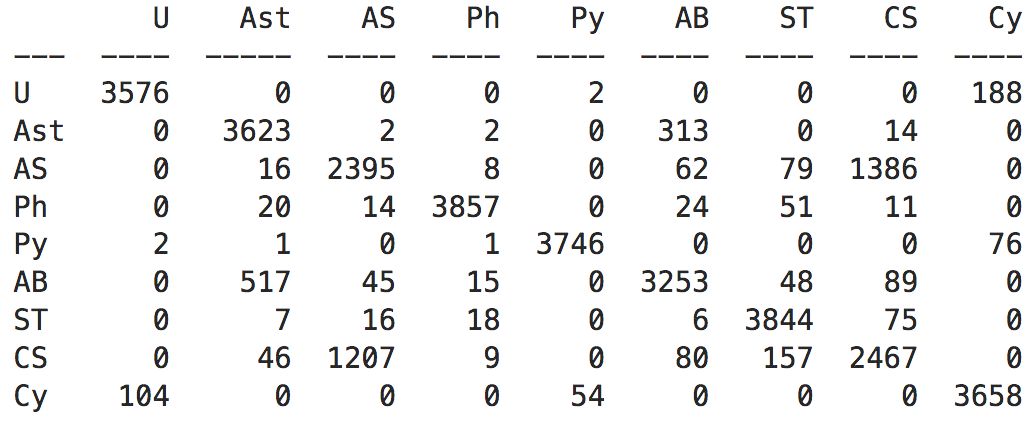
\includegraphics[width=\linewidth]{figs/rf_confusion_matrix.png}
			\caption{Confusion Matrix for Random Forest}
		\end{figure}
		
		U: Urethritis,  Ast: Asthma,  AS: Acute Sinusitis,  Ph: Pharyngitis, \\
		Py: Pyelonephritis,  AB: Acute Bronchitis,  ST: Strep. Throat,\\
		CS: Chronic Sinusitis,  Cy: Cystitis
	\end{frame}
	
		\subsection{Naive Bayes}
		\begin{frame}
			\frametitle{Model Evaluation: Naive Bayes on Symcat-Synthea}
			\begin{itemize}
				\item But the Random Forest is not the only appropriate model
				\item Naive Bayes is also a valid choice in this case
				\item Assumes conditional independence for the attributes once the disease is known
				\item Disease condition the only thing responsible for the presented symptoms
				\item Does not model possible relationships between symptoms, e.g perhaps sneezing is more likely to occur if a cough is present
				\item But despite this strong assumption, given enough data, Naive Bayes is a good classifier
				\item Obtained 88.0\% accuracy on both the train set and the hold out test data.
			\end{itemize}
		\end{frame}
	
		\begin{frame}
			\frametitle{Model Evaluation: Naive Bayes on Symcat-Synthea}
			\begin{figure}
				\includegraphics[width=0.8\linewidth]{figs/naive_bayes_learning_curve.pdf}
				\caption{Learning Curve (Accuracy) for Naive Bayes}
			\end{figure}
		\end{frame}
	
		\begin{frame}
			\frametitle{Model Evaluation: Naive Bayes on Symcat-Synthea}
			\begin{figure}
				\includegraphics[width=0.8\linewidth]{figs/naive_bayes_learning_auc_curve.pdf}
				\caption{Learning Curve (Average AUC) for Naive Bayes}
			\end{figure}
		\end{frame}
	
		\begin{frame}
			\frametitle{Model Evaluation: Naive Bayes on Symcat-Synthea}
			\begin{figure}
				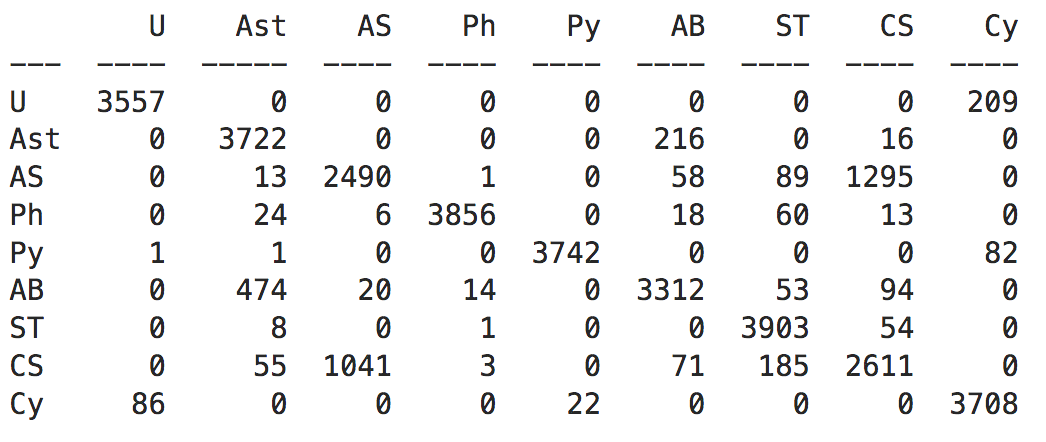
\includegraphics[width=\linewidth]{figs/naive_bayes_confusion_matrix.png}
				\caption{Confusion Matrix for Naive Bayes}
			\end{figure}
			
			U: Urethritis,  Ast: Asthma,  AS: Acute Sinusitis,  Ph: Pharyngitis, \\
			Py: Pyelonephritis,  AB: Acute Bronchitis,  ST: Strep. Throat,\\
			CS: Chronic Sinusitis,  Cy: Cystitis
		\end{frame}

\section{Next Steps}
\begin{frame}
\frametitle{Next Steps}
\begin{itemize}
	\item From confusion matrix, the errors were from very \textit{similar} conditions with overlapping symptoms
	\item One idea is to also augment the data with features that would make such distinction possible
	\begin{itemize}
		\item VAS scores for symptom intensity
		\item Duration of symptom
		\item Body localization of symptom, e.t.c
	\end{itemize}
	\item Extend analysis to full Symcat-Synthea dataset i.e all 801 conditions and 474 symptoms
	\item Data standardization to allow for easy integration with other data sources e.g MIA
\end{itemize}
\end{frame}

\begin{frame}
\frametitle{Next Steps}
\begin{itemize}
	\item Naive Bayes is a good classifier with enough data, but bad estimator and hence not ideal for differential diagnosis
	\begin{itemize}
		\item A generative modeling using a Multivariate Bernoulli distribution might be a better idea
	\end{itemize}
	\item So far, classification has been performed, but differential diagnosis is the aim
	\begin{itemize}
		\item How to evaluate a differential diagnosis?
		\item We are only sure of what the most likely condition is.
		\item How to rank what the $n$ most likely conditions should be?
		\item Select metric for evaluating the differential diagnoser
	\end{itemize}
\end{itemize}
\end{frame}
%------------------------------------------------

\begin{frame}
\Huge{\centerline{The End}}
\end{frame}

%----------------------------------------------------------------------------------------

\end{document} 